\chapter{Design and Implementation}

(approx. 10 pages)\\
* Approach to design\\
* important issues and choices and their relationships to theoretical concepts and the hardware and software platforms\\
* You can use one subsection for the driver and another for the data logger.\\

* Check if you have addressed Provided a graphical representation for your design?\\
* Provided a Project folders and files diagram?\\
* Did you use the GPIO module? How?\\
* Did you use the graphics library? How?\\
* Did you use interrupts? How?\\
* Did you use multiple threads / handlers? How? Why?\\
* Did you use the ADC? How? Did you use TI-RTOS? How?



\begin{figure}[H]
	\begin{center}
		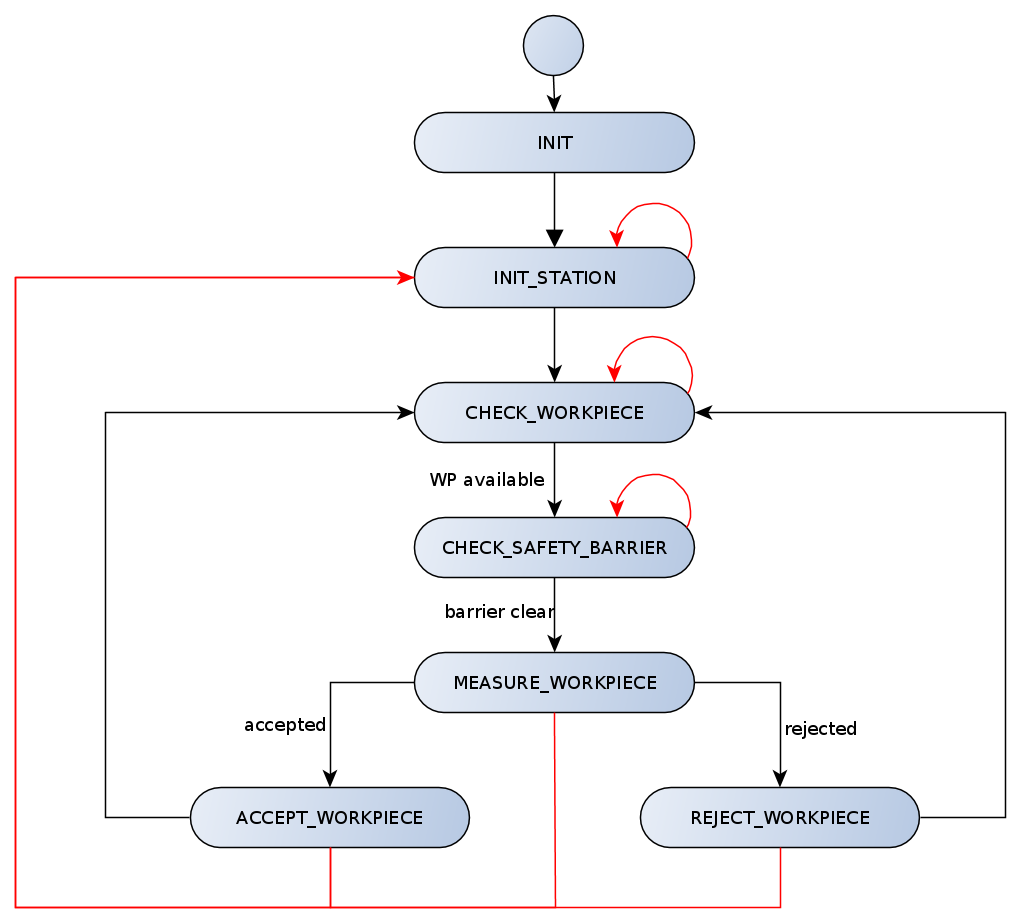
\includegraphics[scale=.50]{media/StateMachine_Main.png} 	
		\caption{Main State Machine}
		\label{fig:statemachine}
	\end{center}
\end{figure}



\begin{figure}[H]
	\begin{center}
		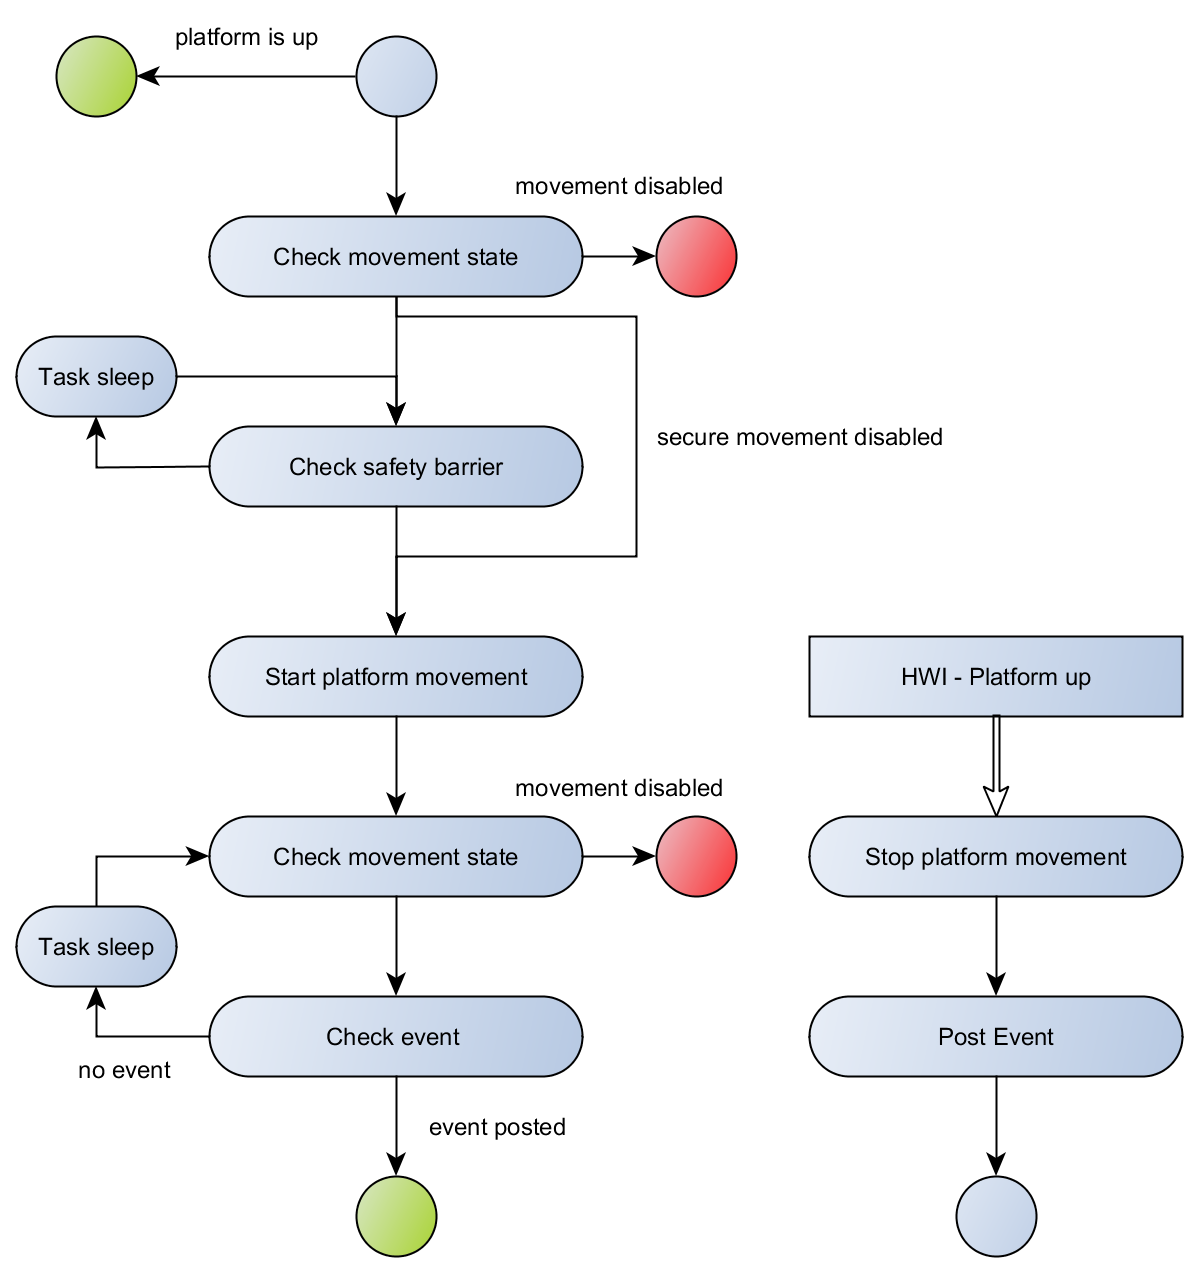
\includegraphics[scale=.40]{media/Flow_Chart_MovePlatform.png} 	
		\caption{Flow Chart Move Platform}
		\label{fig:moveplatform}
	\end{center}
\end{figure}